\section{Deposit}



\begin{figure}[h!]
  \begin{sequencediagram}
    \newinst{wallet}{\shortstack{Customer wallet \\
      \\ 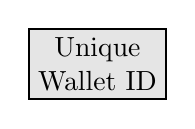
\begin{tikzpicture}
        \node [fill=gray!20,draw=black,thick,align=center] { Unique \\ Wallet ID};
      \end{tikzpicture}
    }}
    \newinst[2]{exchange}{\shortstack{Taler (exchange) \\
       \\ \begin{tikzpicture}[shape aspect=.5]
        \tikzset{every node/.style={cylinder,shape border rotate=90, draw,fill=gray!25}}
        \node at (1.5,0) {\shortstack{{{\tiny Database}}}};
       \end{tikzpicture}
    }}
    \newinst[2]{bank}{\shortstack{Customer bank \\
      \\ 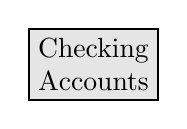
\begin{tikzpicture}
        \node [fill=gray!20,draw=black,thick,align=center] {Checking \\ Accounts};
      \end{tikzpicture}
    }}
    \postlevel
    \begin{callself}{wallet}{Review deposit fees}{}
    \end{callself}
    \mess[0]{wallet}{Deposit {(Coins)}}{exchange}
    \begin{sdblock}{Acceptable account?}{}
    \mess[0]{exchange}{{Refuse deposit}}{wallet}
    \end{sdblock}
    \begin{sdblock}{KYC/AML required?}{}
    \begin{callself}{exchange}{Figures~\ref{fig:proc:kyc}, \ref{fig:proc:aml}}{}
    \end{callself}
    \end{sdblock}
%    \prelevel
%    \prelevel
%    \begin{sdblock}{User abort?}{}
%    \mess[0]{wallet}{{Request abort}}{exchange}
%    \mess[0]{exchange}{{Abort confirmation}}{wallet}
%    \end{sdblock}
    \mess[0]{exchange}{{Initiate transfer}}{bank}

\end{sequencediagram}
  \caption{Deposit interactions between customer, Taler exchange (payment
    service provider) and customer's bank.}
  \label{fig:int:deposit}
\end{figure}

We do {\bf not} permit the customer to regain control over their funds {\em
  unless} they pass the KYC/AML checks. The technical reason is simply that
the KYC/AML checks happen {\em after} the aggregation logic and at this point
refunds are no longer permitted.  From a compliance perspective, this also
prevents malicious customers from risk-free probing of the system.
